% Relatório desenvolvido para a matéria programação natural
% Segundo Trabalho
% Mestrado IC-UNICAMP
% Novembro 2008
% Author: Thiago Alvarenga Lechuga (thiagoalz@gmail.com)
% IC-UNICAMP
% http://www.ic.unicamp.br/~079699
%


\documentclass{acm_proc_article-sp}
%\documentclass[a4paper,10pt]{article}

\usepackage[utf8]{inputenc}
\usepackage{textcomp}

\begin{document}

\title{Relatório de projeto computacional}
\subtitle{Computação Bio-inspirada em Otimização Contínua e Discreta}

\numberofauthors{1}

\author{
% You can go ahead and credit any number of authors here,
% e.g. one 'row of three' or two rows (consisting of one row of three
% and a second row of one, two or three).
%
% The command \alignauthor (no curly braces needed) should
% precede each author name, affiliation/snail-mail address and
% e-mail address. Additionally, tag each line of
% affiliation/address with \affaddr, and tag the
% e-mail address with \email.
%
% 1st. author
\alignauthor
Thiago A. Lechuga\\
    \affaddr{RA079699}\\
       \affaddr{Instituto de Computação, Universidade Estadual de Campinas}  \\
       \affaddr{Campinas, São Paulo, Brasil}\\
       \email{thiago.lechuga@students.ic.unicamp.br}
}

\maketitle

\begin{resumo}
O objetivo desse trabalho computacional é utilizar conceitos e ferramentas vistos em sala para tratar problemas de interesse prático.

O trabalho é composto por um sucinto referencial teórico seguido por aplicações praticas de ACO min-max, algorítimo Genético, simulated annealing, PSO, opt-aiNet,aiNet, ARIA e comparações entre os três primeiros algoritmos e o Concorde. Para cada aplicação o trabalho demostra as técnicas, ferramentas e dados utilizados, seguidos pelos resultados.
\end{resumo}


\section{Implementação}
Nessa sessão os algoritmos desenvolvidos serão apresentados. Para cada algoritmo temos uma subseção com a descrição do problema, detalhes de implementação e resultados.
Na primeira parte, o problema de TSP será resolvido com diversos algoritmos diferentes - ACO, AG e Simulated annealing -, em seguida será apresentado um breve resumo de características do Concorde, e após uma comparação de todos os algoritmos. Por fim serão apresentados os três métodos imuno-inspirados implementados: opt-aiNet,aiNet e ARIA.

Todas as instâncias de TSP foram retiradas do TSPLib \cite{TSPLIB} ; a base ulysses22 para uma instância fácil, a eil51 como média e a pr439 como difícil.

\subsection{ACO min-max}
Para resolver o problema do TSP com ACO utilizei a biblioteca para ACO do grupo IRIDIA \cite{ACO-IRIDIA} com o intuito de abstrair a implementação de partes da modelagem, como o "grafo" que as formigas devem percorrer, e me preocupar apenas com com a implementação específica do algoritmo.

Trabalhar com essa biblioteca foi bem desapontador. Ela é toda desenvolvida em C em com programação estruturada, não possui ferramentas de auxílio gráfico e não foi planejada para ser extensível. O código é bem comentado (E mantive o mesmo padrão nas atualizações), mas a estrutura procedural tornou o ato de fazer modificações um trabalho árduo e a legibilidade do código ficou prejudicada. Ainda assim a biblioteca ofereceu diversas ferramentas que colaboraram bastante com o desenvolvimento do projeto como a leitura de arquivos, parse das entradas da linha de comando e outros. O uso de algumas ferramentas dessa biblioteca também colaborou com os bons resultados apresentados pelo ACO.

Como o código foi todo em C, tive dificuldade em implementar uma interface gráfica, então o programa é todo acessado por linha de comando e para plotar os gráficos com os resultados utilizei a saída do ACO como entrada para a parte gráfica dos outros algoritmos, desenvolvidos em Java.

Na implementação foi utilizado um modelo de grafo completo com os feromônios sendo aplicados nas arestas. Inicialmente o algoritmo calcula as distâncias de todas as arestas para montar a matriz do grafo. O limites min e max podem ser vistos na função "checkPheromoneTrailLimits" no arquivo "ants.c" e foi usado um fator de evaporação de "0.5". Como termo heurístico foi utilizada a distância para a próxima cidade com uma influencia duas vezes maior que a do feromônio (numero em que foram obtidos melhores resultados).

O programa ficou dividido em 4 arquivos principais:

\begin{itemize}
	\item \textbf{acotsp.c:} Principais rotinas do protocolo.
	\item \textbf{ants.c:} Comportamento das formigas.
	\item \textbf{TSP.c:} Funções específicas de TSP.
	\item \textbf{parse.c:} Funções para efetuar o parse das instruções enviadas pela linha de comando.
\end{itemize}

Para usar o software basta descompactar o arquivo, entrar na pasta pelo console de comando e digitar "./acotsp -i arquivo.tsp -m qtdFormigas". A quantidade de formigas padrão usadas nos testes foi 25.

\subsubsection{Avaliação dos Resultados}
Para a instância fácil foi usado o arquivo "DadosTsp/facil-ulysses22-TSPLIB.tsp". Foi observado que para esse caso os limites de min-max não tiveram grande influência; com ou sem os limites o algoritmo encontrou o caminho ótimo (Também encontrado pelo concorde) em menos de 1 segundo e na primeira iteração. Esse comportamento foi bastante influenciado pelo termo heurístico. A distância final foi de 72 e os resultados estão no arquivo "resultados/facil-ACO".A figura ~\ref{fig:facil-concorde} exibe o caminho encontrado.

\begin{figure}[ht]
 \begin{center}
  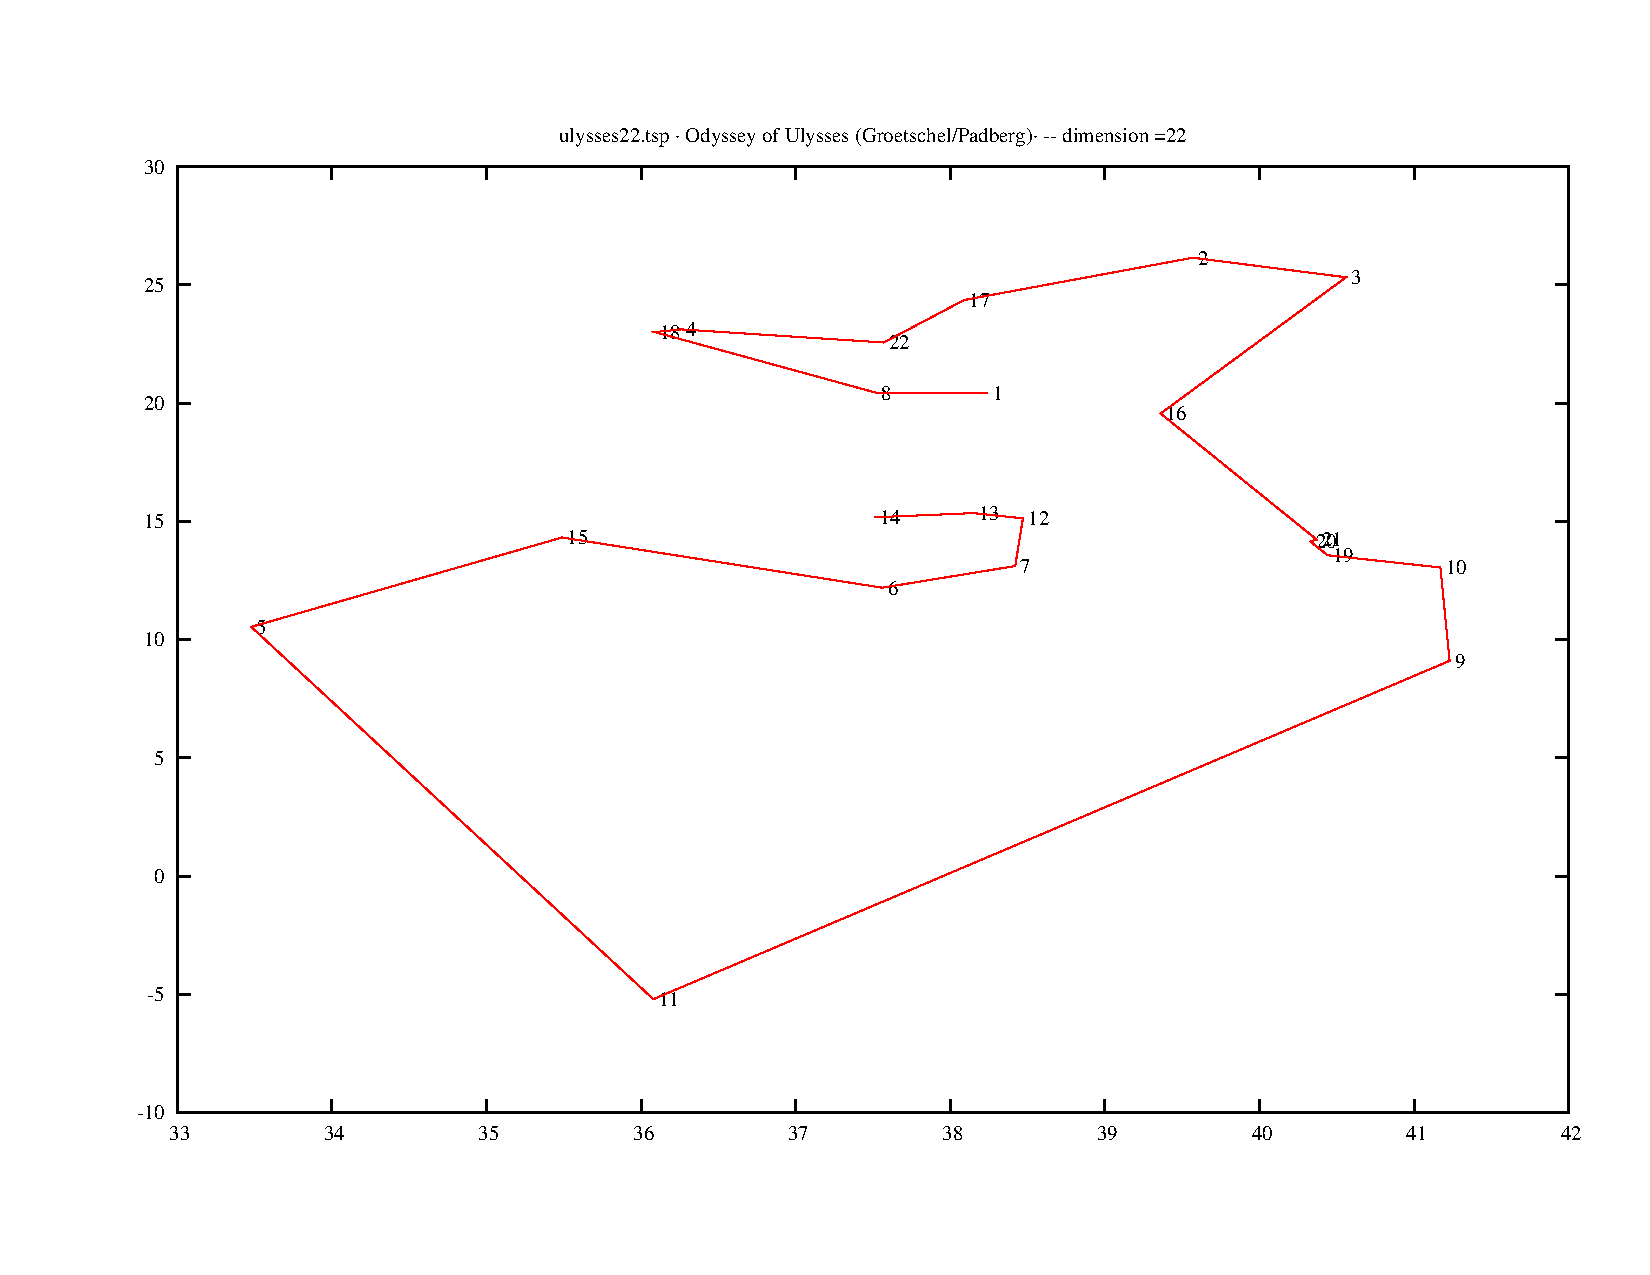
\includegraphics[scale=0.3]{imagens/facil_concorde.pdf} 
  \caption{Resultado ótimo para a instância fácil de TSP}
  \label{fig:facil-concorde}
 \end{center}
\end{figure}

Para a instância mediana foi usado o arquivo "DadosTsp/medio-eil51-TSPLIB.tsp". Foi observado um comportamento semelhante a instância fácil pois, apesar de ser um pouco mais complexa, escolher a cidade mais próxima era uma boa escolha na maioria das vezes e por isso o termo heurístico teve grande peso nos resultados. Para evitar isso a instância difícil foi escolhida cuidadosamente. Mas já foi possível verificar uma boa diferença, a quantidade média de iterações para encontrar a melhor resposta subiu para 1.7 e o tempo sem os limites min e max foi dez vezes maior. A  distância final foi de 426 e os resultados estão no arquivo "resultados/medio-ACO".A figura ~\ref{fig:medio-concorde} exibe o caminho encontrado.

\begin{figure}[ht]
 \begin{center}
  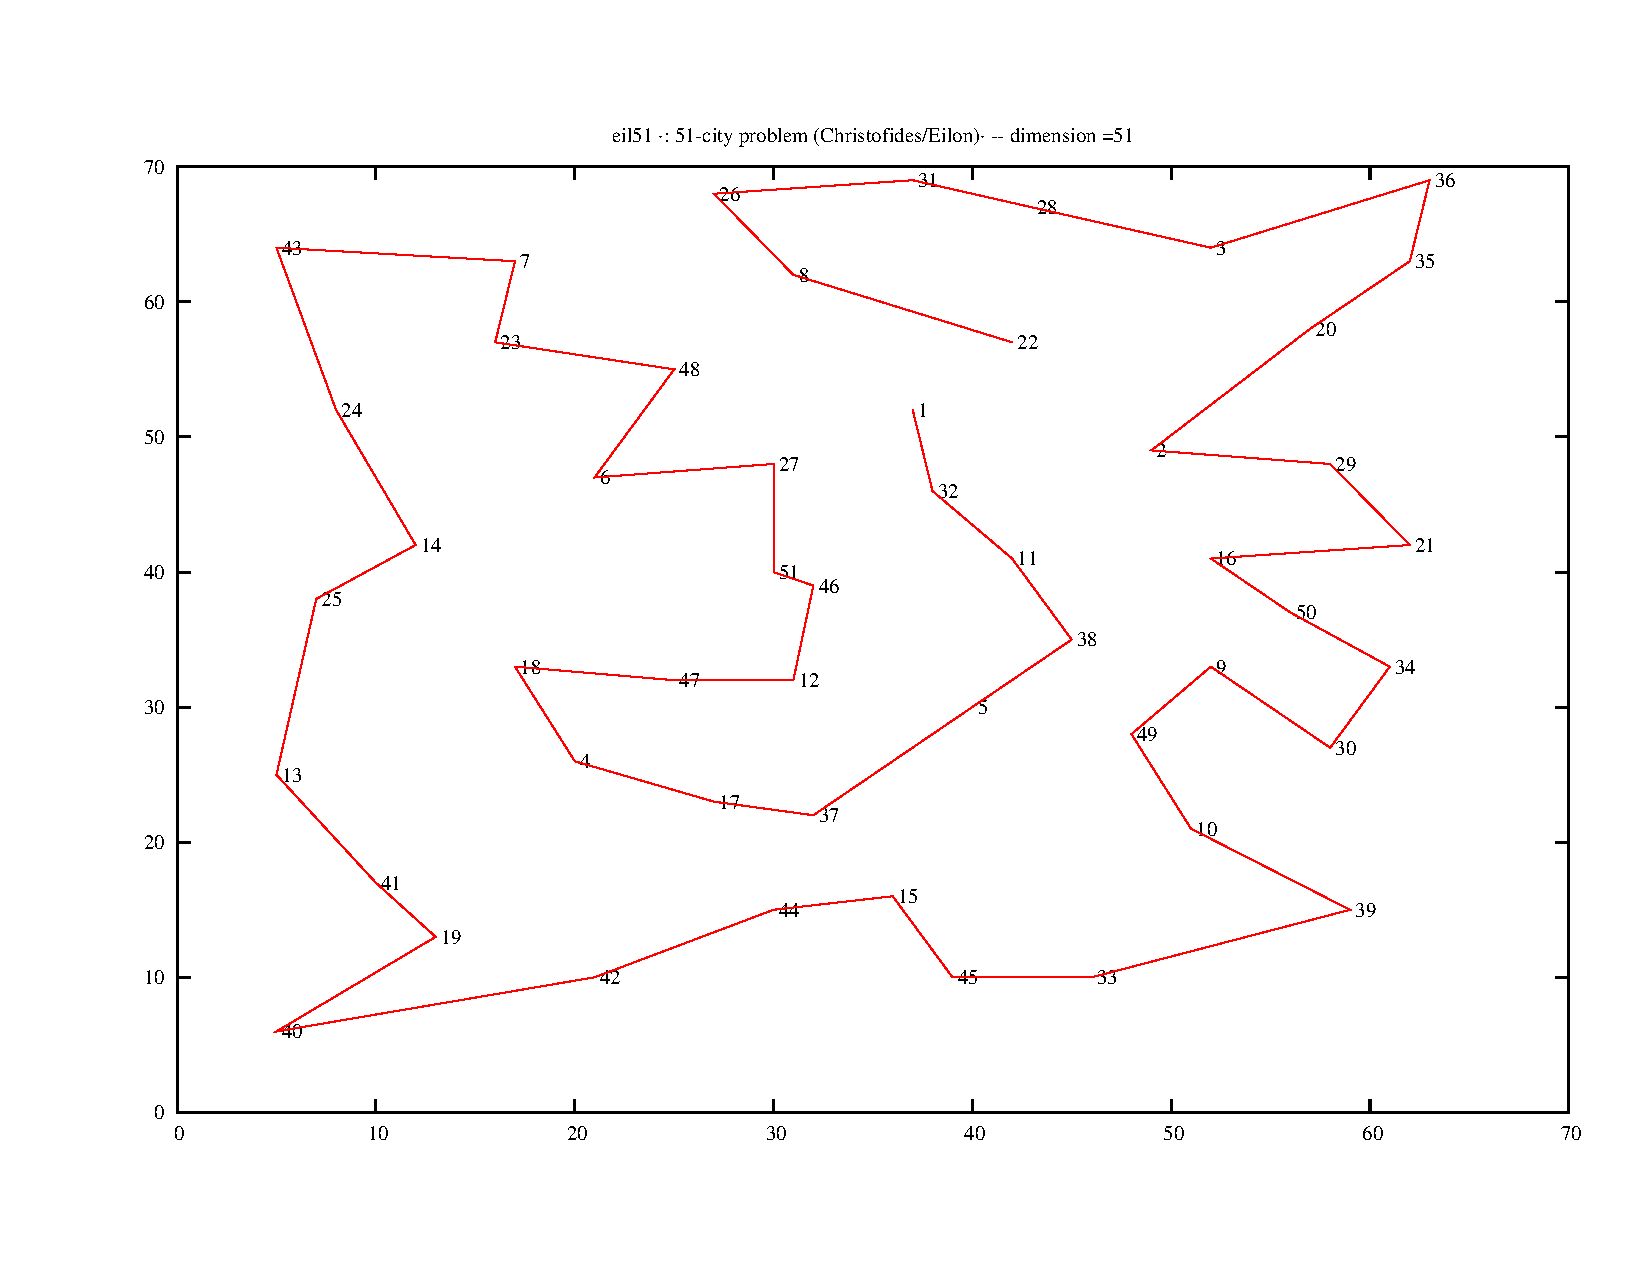
\includegraphics[scale=0.3]{imagens/medio_concorde.pdf} 
  \caption{Resultado ótimo para a instância média de TSP}
  \label{fig:medio-concorde}
 \end{center}
\end{figure}

Para a instância difícil o arquivo usado foi o "DadosTsp/dificil-pr439-TSPLIB.tsp". Para instâncias desse porte o ACO se mostrou com os melhores resultados, mais uma vez só perdendo para o concorde. O melhor resultado conhecido é o visto na figura ~\ref{fig:medio-concorde} com tamanho 107217. Com aproximadamente 25 segundos e pouco mais de 150 iterações o algoritmo foi capaz de encontrar caminhos muito próximos do Concorde com pequenas diferenças no trajeto, quase que imperceptíveis no gráfico, e com tamanho 107881 em média. Para a execução sem os limites max e min os resultados foram bem inferiores.


\subsection{Algoritmo Genético}
Nessa etapa do trabalho tinha-se como objetivo implementar um algoritmo genético para resolver problemas de TSP com propostas de busca local. Para evitar os problemas da etapa anterior tive maior cuidado na busca por ferramentas que poderiam auxiliar a implementação do projeto. Utilizei então duas ferramentas de apoio: A biblioteca JGAP \cite{JGAP} para facilitar a estruturação e extensibilidade da aplicação e a biblioteca JFreeChart\cite{JFreeChart} para plotar os gráficos com os caminhos do TSP, ambas para a linguagem Java.

A implementação foi toda orientada a objetos. A biblioteca JGAP facilitou bastante a implementação e permitiu que o código ficasse melhor estruturado do que se eu mesmo fosse modelar a aplicação em um curto período de tempo. O código ficou bem legível, facil de alterar e extensível, contudo as vantagens ficaram por aí. Apesar se já existir a estrutura de um gene por exemplo, é necessário especificar o formato do gene e do cromossomo específico para a aplicação, além dos algoritmos de fitness, crossover, mutação, seleção e busca local. Essa abordagem também prejudicou a velocidade da aplicação. A biblioteca JFreeChart facilitou a plotagem dos gráficos, porém se mostrou muito lenta e inviabilizou constantes atualizações dos gráficos.

A função de fitness usada pode ser vista na classe SalesmanFitnessFunction.java. Ela é bem simples, o maior inteiro possível de se representar em java foi definido como o pior resultado possível (Integer.MAXVALUE) e zero o melhor, então simplesmente calcula-se a distancia total do percurso (incluindo a volta) e o fitness resultante é dado por: (Integer.MAXVALUE / 2) - distanciaTotal;

Os algoritmos de crossover e mutação implementados foram os vistos em sala de aula e se encontram respectivamente nas classes Crossover.java e SwappingMutationOperator.java. O algoritmo de seleção pode ser escolhido entre roleta e torneiro mas o segundo foi utilizado para todos os testes por gerar melhores resultados (testado experimentalmente).

Para a implementação das buscas locais foi utilizado o padrão de projeto AbstractFactory, permitindo configurar o TSP com a busca desejada (Configurável pela tela inicial). Duas buscas foram implementadas A primeira consistia em apenas trocar aleatoriamente a ordem de duas cidades adjacentes e testar se o caminho tinha melhorado até acertar alguma vez. Esse método melhorou os resultados, mas verifiquei que o custo computacional era muito alto e vislumbrei uma abordagem potencialmente melhor. Não cheguei a verificar na literatura por alternativas mas a minha idéia para implementar a segunda busca local foi baseada na figura ~\ref{fig:grafo}, onde podemos ver que um cruzamento "sempre" é uma escolha ruim e busca-los e eliminá-los melhora o algoritmo além de não ser necessário testar continuamente se ouve melhora, já que sempre há melhora. Então o algoritmo segue buscando cruzamentos e retira o primeiro que encontra. Na figura ~\ref{fig:grafo} tento mostrar que não importa a configuração do grafo, eliminar um cruzamento sempre irá diminuir a rota.

\begin{figure}[ht]
 \begin{center}
  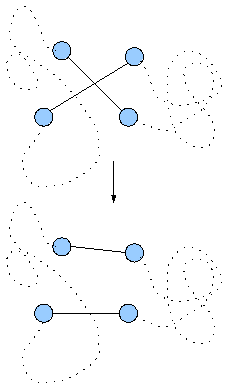
\includegraphics[scale=0.5]{imagens/grafo.png} 
  \caption{Exemplo de um cruzamento retirado de um grafo genérico}
  \label{fig:grafo}
 \end{center}
\end{figure}

O programa ficou então dividido em 8 classes principais:

\begin{itemize}
	\item \textbf{controle.GA.TSP:} Define o comportamento geral do algoritmo e garante a estrutura dos cromossomos
	\item \textbf{controle.GA.Alelo:} Definindo um alelo, basicamente cada alelo representa uma cidade.
	\item \textbf{controle.GA.GeneTSP:} Define um gene para o TSP composto por uma alelo especifico para TSP.
	\item \textbf{buscaLocal.BuscaLocalCruzamento:} Executa a busca local retirando cruzamento de um dado GeneTSP.
	\item \textbf{buscaLocal.BuscaLocalTroca:} Executa a busca local trocando alelos de um dado chromosome composto por GeneTSP.
	\item \textbf{Crossover.java:} Algoritmo de Crossover.
	\item \textbf{SwappingMutationOperator.java:} Algoritmo de mutação.
	\item \textbf{SalesmanFitnessFunction.java:} Algoritmo da função de Fitness.
\end{itemize}

Para executar o programa a maquina virtual Java é necessária. Em seguida basta digitar "java -jar programa-ga.jar". Na figura ~\ref{fig:telaGA} vemos a tela principal do programa. Para utiliza-lo basta configurar os parâmetros: População, Gerações, Passo (De quantas em quantas gerações deve-se plotar o gráfico com o resultado atual.), Algoritmo de seleção, algoritmo de busca local e arquivo de dados. Em seguida basta executar.
O programa ficou com um pequeno problema de memória que não tive tempo de arrumar, só é possível executar uma vez o GA, depois é necessário fechar o programa e abrir novamente.

\begin{figure}[ht]
 \begin{center}
  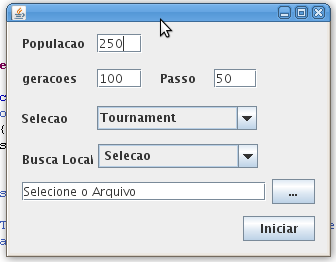
\includegraphics[scale=0.5]{imagens/ga_telaprincipal.png} 
  \caption{Tela principal do programa de Algoritmo Genético}
  \label{fig:telaGA}
 \end{center}
\end{figure}

\subsubsection{Avaliação dos Resultados}
Para a instância fácil foi usado o arquivo "DadosTsp/facil-ulysses22-simples.tsp". Mesmo para a instância simples o sistema não foi capaz de encontrar o resultado ótimo (tamanho 72) mas conseguiu melhorar bastante do caminho inicial (tamanho 138), visto na figura ~\ref{fig:facilGA1}, para bem próximo do resultado ótimo (tamanho 85), visto na figura ~\ref{fig:facilGA2}. Os melhores resultados foram obtidos usando o algoritmo de busca local "BuscaLocalCruzamento", esses resultados foram na média 18\textdiscount melhores do que sem busca local. Foram utilizadas 200 indivíduos, o ganho adicionando mais indivíduos era muito pequeno; e 100 gerações, mais que isso a diversidade não era suficiente para progredir. Tempo médio para encontrar o melhor resultado foi de 2.4 minutos.

\begin{figure}[ht]
 \begin{center}
  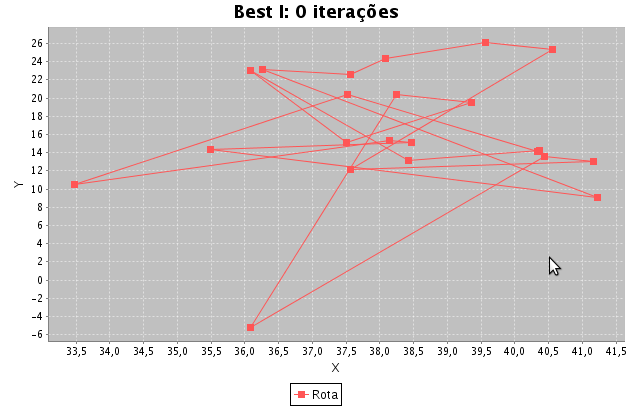
\includegraphics[scale=0.4]{imagens/facil_GA1.png} 
  \caption{Solução para TSP gerada randomicamente na primeira geração do GA (instância fácil)}
  \label{fig:facilGA1}
 \end{center}
\end{figure}

\begin{figure}[ht]
 \begin{center}
  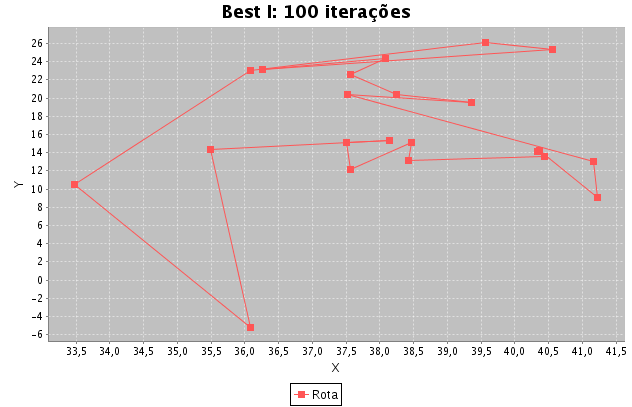
\includegraphics[scale=0.4]{imagens/facil_GA2.png} 
  \caption{Melhor solução para TSP gerada após 100 gerações do GA (instância fácil)}
  \label{fig:facilGA2}
 \end{center}
\end{figure}

Para a instância de dificuldade média foi usado o arquivo "DadosTsp/medio-eil51-simples.tsp".  O algoritmo foi configurado com 1000 indivíduos e 1000 gerações. Após aproximadamente 5 minutos  de execução o melhor resultado obtido foi o exibido na figura ~\ref{fig:medioGA2}. Esse resultado teve um tamanho de 700, mais de 60\textdiscount menor do que o gerado aleatoriamente (figura ~\ref{fig:medioGA1})  e 22\textdiscount melhor do que os gerados sem busca local (em média), mas ainda distante do ótimo (tamanho 426). 

\begin{figure}[ht]
 \begin{center}
  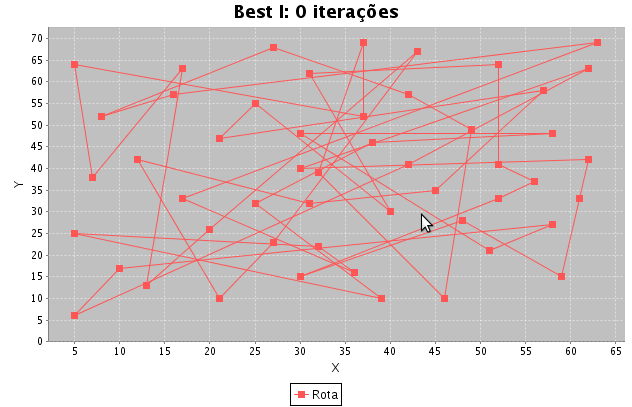
\includegraphics[scale=0.4]{imagens/medio_GA1.png} 
  \caption{Solução para TSP gerada randomicamente na primeira geração do GA (instância média)}
  \label{fig:medioGA1}
 \end{center}
\end{figure}

\begin{figure}[ht]
 \begin{center}
  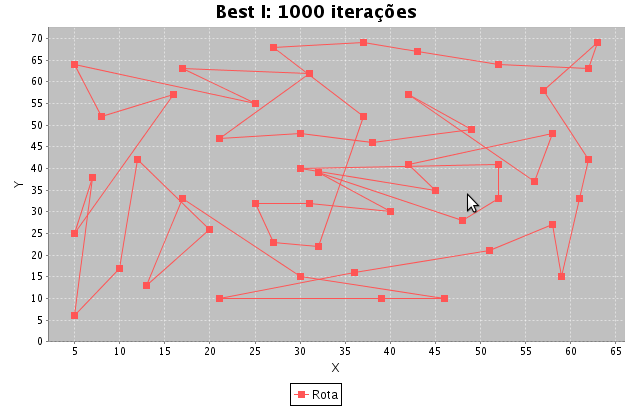
\includegraphics[scale=0.4]{imagens/medio_GA2.png} 
  \caption{Melhor solução para TSP gerada após 100 gerações do GA (instância média)}
  \label{fig:medioGA2}
 \end{center}
\end{figure}


Para a instância difícil o arquivo usado foi o "DadosTsp/dificil-pr439-simples.tsp". Para instâncias desse porte a estrutura escolhida para o GA não foi capaz de resolver os problemas. Mesmo usando populações pequenas, com pouco mais de 2 minutos de execução ocorreram problemas por falta de memória (figura ~\ref{fig:dificilGA}).

\begin{figure}[ht]
 \begin{center}
  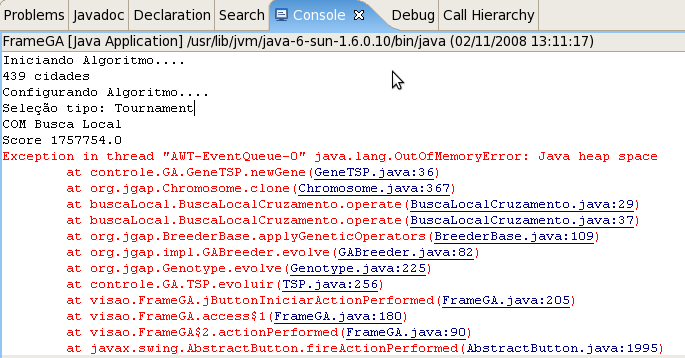
\includegraphics[scale=0.35]{imagens/dificil_GA.png} 
  \caption{Erro por falta de memória do GA executando a instância difícil de TSP}
  \label{fig:dificilGA}
 \end{center}
\end{figure}

Foi observado que um dos motivos para os resultados ruins é que o algoritmo de crossover não está gerando bons descendentes, esse poderia ser melhorado. Outro problema é que o algoritmo de seleção perde muitas vezes indivíduos bons. Ele mantém bem a diversidade, mas poderia ser melhorado para sempre manter alguns dos melhores resultados por exemplo.

\subsection{Simulated Annealing}
Para comparar com os outros algoritmos optei por também resolver TSP com Simulated Annealing.

Por causa da simplicidade do algoritmo e das experiências não muito produtivas com as bibliotecas anteriores, optei por implementar esse algoritmo totalmente em Java e sem nenhuma biblioteca.

O algoritmo ficou mais leve e mais rápido. Contudo não ficou tão bem estruturado e reusável quando o genético. A plotagem dos gráficos também ficou muito mais rápida e permitiu uma flexibilidade maior, contudo ficou simples de mais e sem várias funcionalidades, por exemplo zoom.

O algoritmo foi todo implementado em uma única classe, TSP.java. A execução do algoritmo pode ser vista no método "comp-run-action". Primeiramente a temperatura é iniciada com a distância média entre os pontos do caminho inicial, em seguida roda repetitivamente até atingir a quantidade de steps configurada executando os seguintes passos:

\begin{itemize}
	\item Executa o annealing: repete até o número de tentativas sem melhora ou o número de trocas com melhora (ambos configuráveis) serem atingidos:
		\begin{itemize}
			\item Escolhe aleatoriamente dois pontos para efetuar uma troca.
			\item Se não melhorou volta o anterior.
			\item Se melhorou mantém a troca e aumenta o contador de trocas.
		\end{itemize}
	\item Verifica se obteve melhora. Se obteve reduz a temperatura segundo o fator configurado e repete.
	\item Compara com a melhor rota obtida e substitui se foi melhor.
\end{itemize} 

Lembrando que sempre a melhor solução é mantida. Portanto, executar o algoritmo repetidamente tende a ir melhorando a resposta.

Para executar o programa a maquina virtual Java é necessária. Em seguida basta digitar "java -jar programa-simann.jar". Na figura ~\ref{fig:telaSimAn} vemos a tela principal do programa. Para utiliza-lo basta clicar em executar/propriedades, configurar os parâmetros (mostrados na figura), clicar em arquivo/abrir, selecionar o arquivo desejado e finalmente clicar em executar/run. O melhor resultado obtido é exibido na tela e o tamanho pode ser visto na parte inferior do gráfico.

\begin{figure}[ht]
 \begin{center}
  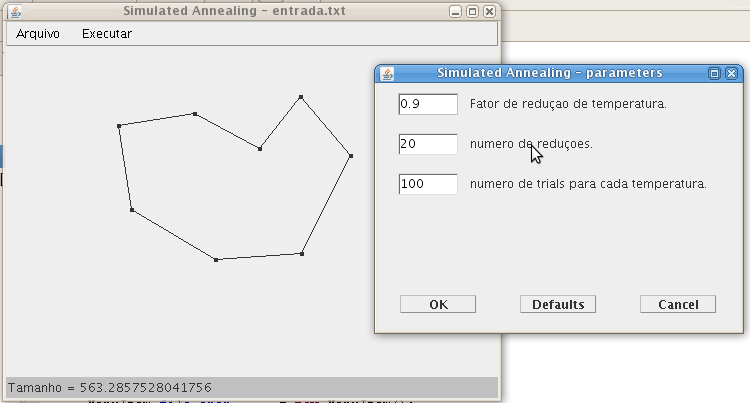
\includegraphics[scale=0.3]{imagens/siman_TSP.png} 
  \caption{Tela principal do programa de Simulated Annealing}
  \label{fig:telaSimAn}
 \end{center}
\end{figure}

\subsubsection{Avaliação dos Resultados}
Como configuração padrão nos testes foram utilizados: Fator de redução de temperatura = 0.9; Número de reduções = 20 e Numero de trials por temperatura = 100. Foi possível verificar que esse foi um dos algoritmos com a melhor relação custo X benefício dos três implementados. Ele foi bem simples de implementar e com pouco tempo de execução conseguiu resultados melhores do o GA, só não mais mais rápido ou eficiente que o ACO.

Para os teste com a instância fácil o arquivo "DadosTsp/medio-eil51-simples.tsp" foi utilizado. Com uma execução já chegou a resultados próximos dos do Genético ( com tamanho = 85). Pela ausência de ferramentas de Zoom tive problemas para plotar os gráficos desse algoritmo Essa instância de TSP possuía pontos muito próximos e ficou impossível de visualizar, por isso não coloquei imagens. Essas poderão ser vistas nas próximas instâncias.

Para o TSP de dificuldade média com poucas execuções já foi possível obter bons resultados , na faixa de 574 de tamanho, com aproximadamente 10 execuções já foi possível obter resultados bem superiores que o do GA, na figura ~\ref{fig:medioSimAn} vemos o melhor resultado gerado (tamanho 482)( o ótimo é de 426). A visualização ficou prejudicada pela falta de uma ferramenta de zoom, como a biblioteca JFreeChart (utilizada no algoritmo de GA) possuía

\begin{figure}[ht]
 \begin{center}
  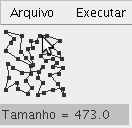
\includegraphics[scale=0.8]{imagens/medio_SimAn.png} 
  \caption{Melhor solução para TSP instância média gerada por Simulated Annealing}
  \label{fig:medioSimAn}
 \end{center}
\end{figure}

Para a instância difícil o arquivo usado foi o "DadosTsp/dificil-pr439-simples.tsp". Para instâncias desse porte o Simulated Annealing se mostrou muito ineficaz. O algoritmo foi sempre muito rápido mas conseguiu melhorar pouco a partir de um caminho aleatório. Os melhores resultados obtidos após diversas execuções consecutivas foram próximos de 328764, sendo que obtido pelo concorde era de 107217. É fácil entender o porquê desse resultado, quando o número de cidades é muito grande, a chance de obter melhora em uma troca é cada vez menor, dessa forma a temperatura acaba caindo muito rapidamente. Para contornar isso deve-se diminuir o fator de redução da temperatura e/ou aumentar o número de tentativas de troca. Contudo, dessa forma o algoritmo fica cada vez mais lento e mesmo assim não obtém bons resultados. Mesmo com configurações bem demoradas os melhores resultados obtidos foram próximos de 200000.

\subsection{Concorde}
Para facilitar e permitir a realização de testes de qualquer local, utilizei a execução do concorde disponível na web pelo servidor NEOS \cite{concorde}. Essa abordagem poupou o tempo de instalação e permitiu que os testes fossem realizados em máquinas onde eu não possuía privilégios de administrador.

O artigo \cite{Hornik2007}  fala sobre soluções eurísticas e exatas para TSP; os autores chamam o concorde de "implementação estado da arte"  e dizem que ele é um dos melhores solucionadores de TSP atualmente disponíveis. \cite{Samuel2003} adiciona que o concorde é o solucionador existente mais rápido para instancias grandes. O concorde inclusive ganhou prêmios em 2001 por solucionar problemas de roteamento de veículos propostos em 1996.

O Concorde suporta diversos tipos de cálculo de distância entre pontos, como distância Euclidiana e Geométrica. Essa opção pode ser configurada no arquivo TSPLIB. Para melhorar a precisão na comparação dos resultados e simplificar a implementação dos algoritmos em todos os testes o cálculo de distância Euclidiana foi utilizado.

\subsubsection{Avaliação dos Resultados}
Para a instância fácil foi utilizado o arquivo "DadosTsp/facil-ulysses22-TSPLIB.tsp" e os resultados são os mesmos visto na imagem ~\ref{fig:facil-concorde} (tamanho=72) que encontram no arquivo "resultados/facil-concorde". Para a instância média foi utilizado o arquivo "DadosTsp/medio-eil51-TSPLIB.tsp", os resultados são os mesmos vistos na imagem ~\ref{fig:medio-concorde}(tamanho=426) e se encontram no arquivo "resultados/medio-concorde". Para a instância difícil, arquivo "DadosTsp/dificil-pr439-TSPLIB.tsp", nenhum outro algorítimo implementado conseguiu resultados tão bons quando o Concorde; esses resultados podem ser vistos na figura ~\ref{fig:medio-concorde}(tamanho=107217) e no arquivo "resultados/dificil-concorde" com mais detalhes. É importante ressaltar que o concorde obteve resultados muito rápidos para todas as instâncias de TSP.

\begin{figure}[ht]
 \begin{center}
  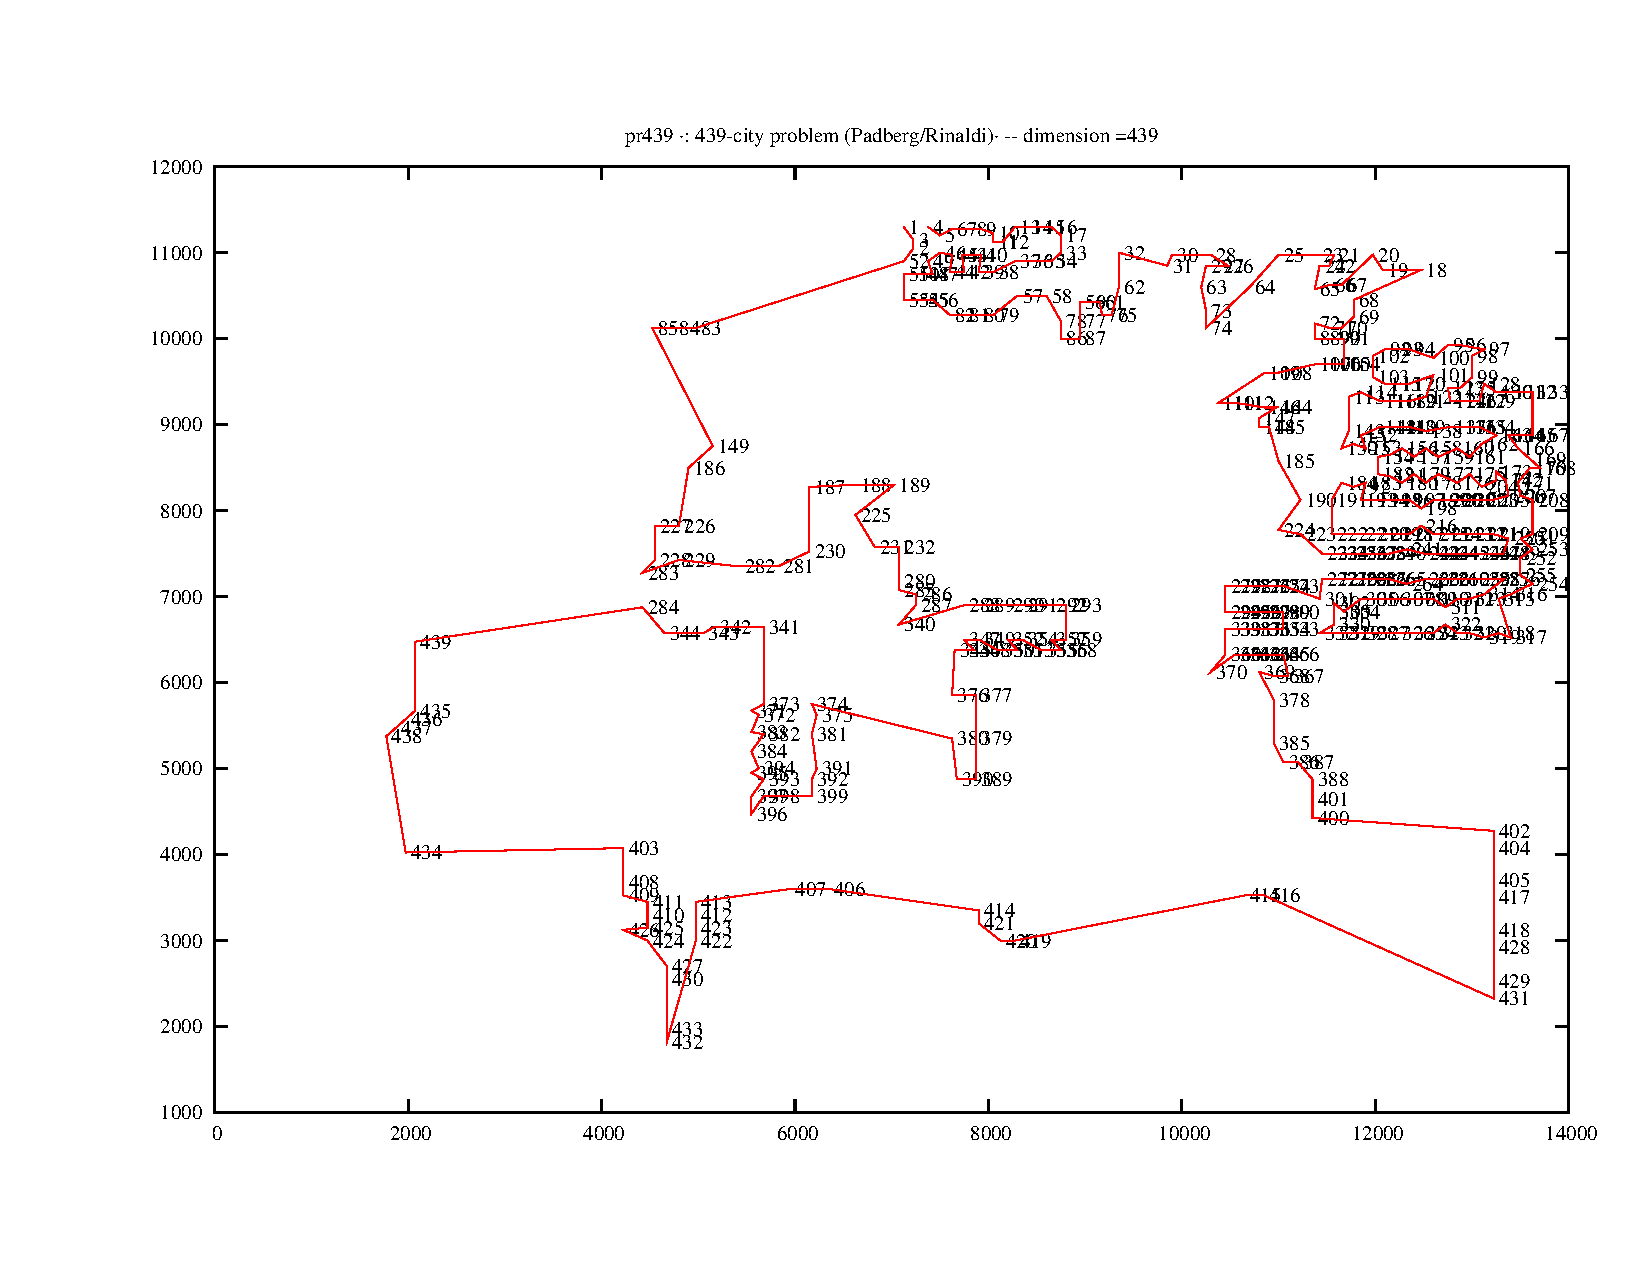
\includegraphics[scale=0.3]{imagens/dificil_concorde.pdf} 
  \caption{Resultado do Concorde para a instância difícil de TSP}
  \label{fig:dificil-concorde}
 \end{center}
\end{figure}

Na próxima sessão iremos comparar os resultados dos algoritmos implementados nesse trabalho entre eles e com o concorde.

\subsection{Comparação entre os algoritmos para TSP}

A tabela mostrada na figura ~\ref{fig:tabela1} mostra, de forma resumida, os dados apresentados nas seções anteriores.

\begin{figure}[ht]
 \begin{center}
  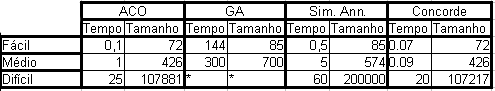
\includegraphics[scale=0.5]{imagens/tabela.png}
  \caption{Tabela resumida com os resultados dos algoritmos de TSP}
  \label{fig:tabela1}
 \end{center}
\end{figure}

\subsection{PSO}
Nessa etapa do projeto o objetivo era otimizar a função "$\displaystyle F(x,y)=x * sen(4 \pi x) - y * sen(4 \pi y + \pi ) + 1$" com PSO. O algorítimo de PSO foi desenvolvido em Java e os gráficos foram plotados usando a ferramenta Octave \cite{octave} (Equivalente ao Matlab para linux), já que não encontrei maneira simples de plotar gráficos 3D em java.

O algoritmo de PSO foi implementado na linguagem Java e completamente orientado a objetos. Foi desenvolvido com vizinhança global e limites de velocidade. Os principais arquivos são:

\begin{itemize}
	\item \textbf{MyPSO.java:} Classe com as funções gerais do PSO. Configurações de velocidade, quantidade de partículas e iterações.
	\item \textbf{MyParticle.java:} Classe com informações das partículas.
	\item \textbf{MyFitnessFunction.java:} Classe que implementa a função a ser maximizada/minimizada. É a responsável por avaliar as partículas.
	\item \textbf{Swarm.java:} Classe que implementa efetivamente o algoritmo de Swarm.
\end{itemize}

Para executar o programa a maquina virtual Java é necessária. Em seguida basta digitar "java -jar programa-pso.jar". Para plotar os gráficos basta executar o arquivo "plotar.octave" no Octave ou no Matlab, substituindo o vetor X pela saída do programa em Java.

\subsubsection{Avaliação dos Resultados}

Com aproximadamente 25 partículas e 100 iterações o algoritmo já foi capaz de encontrar um resultado ótimo na função. Na figura ~\ref{fig:pso-saida} vemos a saída do programa em java e na ~\ref{fig:pso-grafico} vemos esse resultado plotado no gráfico. Os pontos verdes representam as partículas. O algoritmo foi capaz de encontrar um dos picos ótimos sempre que existia um número satisfatório de partículas espalhadas por uma boa área do gráfico inicialmente. Dependendo da organização inicial da partículas o algoritmo convergia para um pico diferente. Quando os limite de velocidade são retirados as partículas até passam pelo ótimo, mas acabam passando pela velocidade muito alta e acabam se concentrando nas extremidades do gráfico.

\begin{figure}[ht]
 \begin{center}
  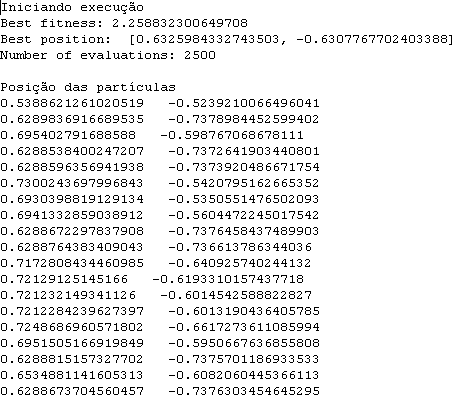
\includegraphics[scale=0.5]{imagens/pso-saida.png}
  \caption{Saida do algoritmo de PSO}
  \label{fig:pso-saida}
 \end{center}
\end{figure}

\begin{figure}[ht]
 \begin{center}
  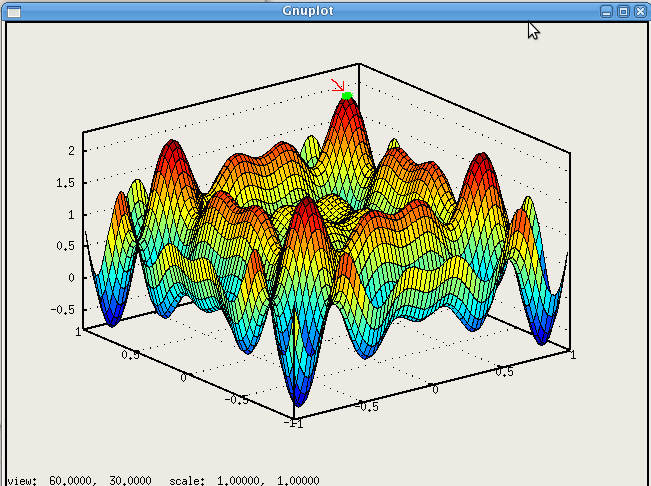
\includegraphics[scale=0.35]{imagens/pso-grafico.png}
  \caption{Resultados do PSO plotados com o Octave}
  \label{fig:pso-grafico}
 \end{center}
\end{figure}

Como o algoritmo foi implementado com vizinhança global, todas as partículas convergem para o mesmo pico. Não tive tempo hábil de implementar vizinhança local, mas provavelmente com esse tipo de implementação seria possível identificar vários picos.

\subsection{opt-aiNet}
Nessa etapa do projeto o objetivo era otimizar a função "$\displaystyle F(x,y)=x * sen(4 \pi x) - y * sen(4 \pi y + \pi ) + 1$" com opt-aiNet. De forma similar ao PSO, o algorítimo de opt-aiNet foi desenvolvido em Java e os gráficos foram plotados usando a ferramenta Octave \cite{octave}.

O algoritmo de opt-aiNet foi implementado na linguagem Java e orientado a objetos, baseado nos códigos explicados em \cite{aisweb}.Os principais arquivos são:

\begin{itemize}
	\item \textbf{Main.java:} Classe com as funções gerais do algoritmo. Inicialização e parâmetros de configuração.	
	\item \textbf{OptFunction.java:} Classe que implementa a função a ser maximizada/minimizada. É a responsável por avaliar.
	\item \textbf{NetworkCell.java:} Classe que implementa o comportamento das network cells.
	\item \textbf{OptAinet.java:} Classe que implementa efetivamente o Opt-aiNet.
\end{itemize}

Para executar o programa a maquina virtual Java é necessária. Em seguida basta digitar "java -jar programa-optainet.jar". Para plotar os gráficos basta executar o arquivo "plotar.octave" no Octave ou no Matlab, substituindo o vetor X pela saída do programa em Java.

\subsubsection{Avaliação dos Resultados}
Para os testes os seguintes parâmetros foram utilizados:

\begin{itemize}
	\item \textbf{numCells=}20.	
	\item \textbf{numClones=}10.
	\item \textbf{maxIter=}500.
	\item \textbf{suppThres=}0,2.
	\item \textbf{errorThres=}0,001.
	\item \textbf{divRatio=}0,4.
	\item \textbf{mutnParam=}100.	
\end{itemize}

Nos testes foi possível verificar diversas propriedades interessantes do opt-aiNet como a manutenção da diversidade e a auto-adaptação na quantidade de cells. Graças a essas características o sistema foi capaz de identificar os picos quase que na sua totalidade. Na figura ~\ref{fig:optainet} vemos o resultado, onde cada ponto verde representa uma cell.

\begin{figure}[ht]
 \begin{center}
  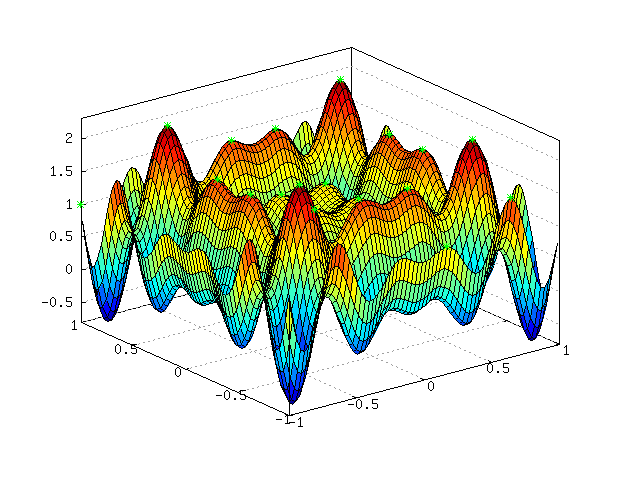
\includegraphics[scale=0.45]{imagens/opt-ainet.png}
  \caption{Resultados do opt-aiNet plotados com o Octave}
  \label{fig:optainet}
 \end{center}
\end{figure}

% \subsection{aiNet}
% descrição do problema:
% 
% ssssss
% 
% resultados
% 
\subsection{ARIA}
O objetivo nessa etapa do projeto era implementar um algoritmo de agrupamento de dados utilizando ARIA. Efetuei tentativas com o Octave e com Java mas mas consegui obter resultados em tempo hábil. O algoritmo para o Octave está com problemas e não consegui concluir o em java. Ambos estão na pasta "ARIA".


% resultados


\section{Conclusões}
%TODO: 
Este trabalho permitiu verificar de maneira prática, os conceitos e características de diversos algoritmos estudados em sala de aula.
TODO: Relembrar os principais comentários dos resultados
% ACO bem rápido e melhores resultados, GA pior em tudo. Concorde imbatível.
% SimAnn Foi possível verificar que esse foi um dos algoritmos com a melhor relação custo X benefício dos três implementados. Ele foi bem simples de implementar e com pouco tempo de execução conseguiu resultados melhores do o GA, só não mais mais rápido ou eficiente que o ACO.
% Concorde é imbatível

\bibliographystyle{abbrv}
\bibliography{bibliografia}

\end{document}